\graphicspath{{sections/06_Cloth_Estimation/}}

%%% Change to your paper title. Can insert line breaks if you wish (otherwise breaks are selected automatically).
\chapter{Extended Kalman Filter for Real-Time State Estimation of Cloth for Robotic Manipulation}\label{sec:cloth}


%%% Change these to your keywords.  Keywords are automatically printed at the end of the abstract.
%%% This command must come BEFORE the end of the abstract.
%%% If you don't want keywords, omit the \keyword{..} command.
% \keywords{Extended Kalman Filter, Robotic Cloth Manipulation, Codimensional IPC Model, AprilTags, State Estimation, Dynamic Textile Interaction, Sim-to-Sim Study, Autonomous Fabric Handling, Cloth Dynamics Simulation, Real-Time Robotic Control}

   
%% Abstract should be no more than 250 words
Robotic cloth manipulation remains constrained by quasi-static assumptions and heuristic-driven strategies, largely due to the absence of fast, accurate state estimation methods. Existing cloth state estimators typically operate at speeds too slow—on the order of several seconds per frame—to capture the highly dynamic behaviors observed in real-world scenarios. While Kalman filtering, particularly the Extended Kalman Filter (EKF), has proven effective for real-time state estimation in robotics, its application to high-dimensional systems like deformable cloth has been underexplored. In this work, we implement an EKF-based framework for cloth state estimation and demonstrate performance at approximately 3 Hz, suggesting that real-time estimation for deformable systems is within reach. To simplify the perception challenge, we instrument the cloth with AprilTags, which reduces the complexity of measurement and node correspondence. We evaluate the robustness of the estimator in a sim-to-sim setting, introducing perturbations such as occlusions and motion blur, and further validate the approach on real cloth using a repeatable motion sequence. Our results indicate that EKF-based estimation offers a promising foundation for enabling closed-loop control and planning for high-dimensional coupled objects manipulation like deformable cloth.


%%%%%%%%%%%%%%%%%%%%%%%%%%%%%%%%%%%%%%%%%%%%%%%%%%%%%%%%%%%%%%%%%%%%%%%%%%%%%%%%%%%%%%%%%%%%%%%%%%%%%%%
%%%%%%%%%%%%%%%%%%%%%  End of fields to be completed. Now write! %%%%%%%%%%%%%%%%%%%%%%%%%%%%%%%%%%%%%%

\section{Introduction}

The dynamic manipulation of cloth represents a significant frontier in robotics, with broad implications for assistive technologies, industrial automation, and healthcare applications~\cite{doumanoglou2014autonomous, maitin2010cloth, erickson2018deep, erickson2018tracking, erickson2020assistive, yu2017haptic}. Beyond convenience, the ability to handle flexible, deformable objects like cloth has the potential to transform daily living, particularly for individuals who require physical assistance.

In the realm of assistive robotics, autonomous systems capable of textile manipulation could enable robotic caregivers to assist the elderly or individuals with disabilities in dressing—supporting independence, privacy, and improved quality of life. Such capabilities could alleviate the reliance on human caregivers for routine dressing tasks and foster greater autonomy for users.

\begin{figure}
\centering
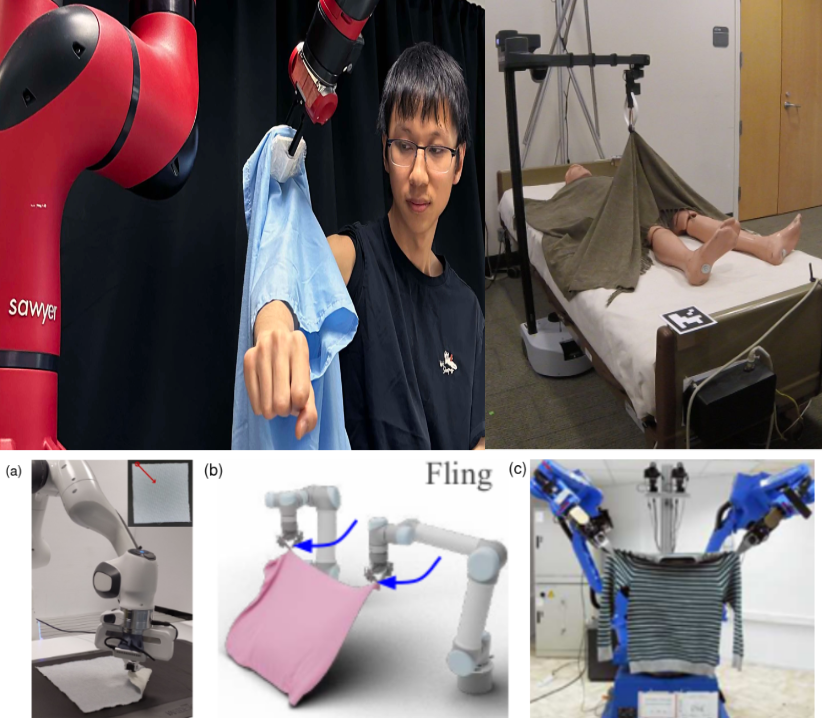
\includegraphics[width=\columnwidth]{CLOTH REPORT PICS/high_level.png}
\caption[Robotic Cloth Manipulation]{(Top left) A robot-assisted dressing system employs a single learned policy to dress various individuals in different poses and garments~\cite{Wang2023One}. (Top right) A mobile manipulator, Stretch RE1, applies a policy trained in simulation to uncover a manikin’s legs with a blanket~\cite{puthuveetil2022bodies}. (Bottom) Demonstrations of action primitives in cloth shaping: (a) Pick-and-Place~\cite{lee2021learning}, (b) Pick-and-Fling~\cite{ha2022flingbot}, and (c) Gravity-based cloth flattening for efficient manipulation in robotic tasks~\cite{doumanoglou2014autonomous}.}
\label{fig:robotic_cloth_manipulation}
\end{figure}

Cloth manipulation also has promising applications in healthcare settings, where robots could assist with repetitive and hygienically sensitive tasks. These include folding sterile garments in operating rooms, changing bed linens, or making beds between patient transitions—all with precision and reduced physical burden on healthcare workers~\cite{seita2019deep}. Such automation could improve hospital efficiency and contribute to better infection control by minimizing unnecessary human contact.

In the industrial domain, advances in robotic cloth manipulation offer transformative potential for the textile and apparel industries. Robots capable of handling deformable materials could automate a wide range of tasks—from fabric cutting and precision measurements to folding, packaging, and even detailed operations like embroidery~\cite{torgerson1988vision}. These systems promise to increase productivity and consistency while allowing human labor to be redirected toward higher-skill, less repetitive work.

Dynamic robotic cloth manipulation poses unique and significant challenges, primarily due to the fundamental differences between deformable materials and rigid bodies. Unlike rigid objects with stable, well-defined geometries, cloth is highly deformable and lacks a fixed shape. It can bend, fold, drape, and wrinkle in complex, often unpredictable ways~\cite{borras2020grasping, sanchez2018robotic}. A single piece of fabric can assume an effectively infinite number of configurations, each shaped by subtle variations in external forces, environmental interactions, and intrinsic properties such as weight, stiffness, and surface texture.

Rigid robotic systems, such as quadrupeds, typically have a relatively low-dimensional state space—on the order of 100 variables. Each rigid body is represented by 13 state parameters: $[x, q, v, \omega]$, where $x$ denotes the 3D position, $q$ the quaternion orientation, $v$ the linear velocity, and $\omega$ the angular velocity. In contrast, cloth possesses an effectively infinite number of degrees of freedom due to its continuous and highly deformable nature. To make state estimation computationally tractable, the cloth is discretized into a finite set of points, each assumed to have no explicit orientation. Despite this simplification, the resulting state space can still involve hundreds or even thousands of parameters, presenting significant challenges for perception and control.

These challenges are further compounded by the limitations of robotic sensing and perception systems, which are primarily designed for rigid-body manipulation. Visual perception can be disrupted by the cloth’s texture, translucency, or self-occlusions, while tactile sensors often fail to capture the global configuration of a deformable object~\cite{tirumala2022learning}. There is also a very challenging node coordination problem that maps the measurement to the discretized model. As a result, effective cloth manipulation requires more advanced algorithms and integrated sensing approaches capable of interpreting the cloth’s high-dimensional and dynamic state.

Conventional manipulation models based on rigid-body dynamics are poorly suited to represent the behavior of textiles~\cite{zheng2024differentiable}. Accurately modeling cloth dynamics across a wide range of conditions remains an open challenge in robotics. Addressing this problem demands progress in fast, high-fidelity modeling, enabling robots to reason about and respond to the inherently unpredictable nature of deformable materials.

% Despite its potential, one of the significant hurdles in cloth manipulation is the accurate estimation of the cloth's state — its position, orientation, and deformation — in real-time. Current methods struggle with state estimation due to the high dimensionality of the problem and the limitations of sensory inputs, which often cannot capture the entire state of the cloth precisely. Techniques like vision-based tracking or direct tactile sensing provide partial solutions but often fall short in complex manipulation scenarios due to occlusions, sensor noise, and the computational complexity of modeling cloth physics accurately.

% On the other hand, cloth simulation presents a unique challenge in robotics and computer graphics due to the inherently complex behavior of fabric materials. Furthermore,Traditional cloth simulators often struggle to authentically replicate complex fabric deformations, leading to unrealistic simulations that fail to mirror the natural draping and folding of actual materials. Many fall short in handling self-collisions and penetrations that occur with cloth dynamics, resulting in less convincing interactions, especially when the cloth folds or layers upon itself. While interactions between cloth and rigid bodies are commonly well-simulated, the more intricate cloth-to-cloth interactions pose a greater challenge, frequently oversimplified by existing models. Additionally, the computational demands of simulating cloth increase with complexity, and simulators may not scale well, nor accurately represent the diverse material properties of different fabrics, impacting the fidelity of the simulation.

The Codimensional Incremental Potential Contact (C-IPC) model offers a significant leap in cloth simulation, employing a $C^2$ constitutive barrier model for complex deformation dynamics and integrated strain limiting to prevent unrealistic stretching, without inducing the numerical artifacts common in traditional methods\cite{Li2020IPC, Li2021CIPC}. It ensures geometrically accurate interactions by robustly modeling the thickness of codimensional objects, enhancing realism in contact scenarios. C-IPC's innovative additive Continuous Collision Detection (ACCD) method resolves collision with high accuracy, crucial for thin materials, while its unified framework seamlessly simulates different geometric codimensions. Collectively, these features render C-IPC a robust tool for stable simulations across a spectrum of conditions, proving essential for advanced applications in robotics and animation. 

Previous works on cloth manipulation or state estimation have largely overlooked the intricacies of cloth physics and rather leverage data-only approaches\cite{clegg2018learning, chen2022efficiently, bertiche2022neural, santesteban2019learning, lahner2018deepwrinkles}. This project addresses the aforementioned challenges by exploring the application of an Extended Kalman Filter (EKF) to estimate the state of cloth accurately. EKFs are well-suited for dealing with the non-linear dynamics typical of cloth behavior, offering a robust framework for fusing model predictions with noisy sensory measurements. Leveraging the advanced physics simulation capabilities of the C-IPC model, we show that fast and certifiable state estimation can be achieved for cloth. We simplify the problem by employing AprilTags — visually recognizable markers — strategically placed across a towel's surface, we can precisely track specific points on a cloth's surface. This tracking data serves as crucial measurement input for our Extended Kalman Filter (EKF).

Our research seeks to fill the gap in dynamic cloth manipulation by enabling more accurate and reliable state estimation, a critical step toward realizing the full potential of robotic systems in interacting with flexible materials. Specifically, this work contributes:

\begin{enumerate}
    \item The first Extended Kalman Filter approach towards cloth state estimation;
    \item The fastest cloth state estimation solution to date;
    \item A sim-to-sim analysis about measurement sparsity and obstructions to analyse robustness of methods;
    \item Real-world demonstrations of cloth state estimation on dynamic cloth behaviors.
\end{enumerate}

\section{Background: Extended Kalman Filters}

The Extended Kalman Filter (EKF) is a recursive estimator for systems governed by nonlinear dynamics and noisy measurements. It extends the Kalman Filter by linearizing the nonlinear models around the current estimate using Jacobians, which makes it especially useful for robotics applications involving deformable objects like cloth, where both motion and perception are highly nonlinear.

We consider the discrete-time system:
\begin{align}
    \mathbf{x}_{k} &= f(\mathbf{x}_{k-1}, \mathbf{u}_{k-1}) + \mathbf{w}_{k-1}, \\
    \mathbf{z}_{k} &= h(\mathbf{x}_{k}) + \mathbf{v}_{k},
\end{align}
where $\mathbf{x}_k$ is the state, $\mathbf{u}_k$ is the control input, and $\mathbf{z}_k$ is the observation. The noise terms $\mathbf{w}_{k-1} \sim \mathcal{N}(0, \mathbf{Q}_{k-1})$ and $\mathbf{v}_k \sim \mathcal{N}(0, \mathbf{R}_k)$ represent process and measurement noise, respectively. The EKF algorithm is shown in Algorithm~\ref{alg:ekf}.
\begin{algorithm}[H]
\caption{Extended Kalman Filter (EKF)}\label{alg:ekf}
\begin{algorithmic}[1]
\Require Previous state estimate $\hat{\mathbf{x}}_{k-1|k-1}$, covariance $\mathbf{P}_{k-1|k-1}$, control input $\mathbf{u}_{k-1}$, measurement $\mathbf{z}_k$, process noise $\mathbf{Q}_{k-1}$, measurement noise $\mathbf{R}_k$
\Ensure Updated state estimate $\hat{\mathbf{x}}_{k|k}$ and covariance $\mathbf{P}_{k|k}$

\Statex \textbf{Predict Step}
\State $\hat{\mathbf{x}}_{k|k-1} \gets f(\hat{\mathbf{x}}_{k-1|k-1}, \mathbf{u}_{k-1})$ \Comment{Propagate state through nonlinear dynamics}
\State $\mathbf{F}_k \gets \left. \frac{\partial f}{\partial \mathbf{x}} \right|_{\hat{\mathbf{x}}_{k-1|k-1}, \mathbf{u}_{k-1}}$ \Comment{Linearize dynamics model}
\State $\mathbf{P}_{k|k-1} \gets \mathbf{F}_k \mathbf{P}_{k-1|k-1} \mathbf{F}_k^\top + \mathbf{Q}_{k-1}$ \Comment{Predict state uncertainty}

\Statex \textbf{Update Step}
\State $\mathbf{y}_k \gets \mathbf{z}_k - h(\hat{\mathbf{x}}_{k|k-1})$ \Comment{Compute measurement residual (innovation)}
\State $\mathbf{H}_k \gets \left. \frac{\partial h}{\partial \mathbf{x}} \right|_{\hat{\mathbf{x}}_{k|k-1}}$ \Comment{Linearize observation model}
\State $\mathbf{S}_k \gets \mathbf{H}_k \mathbf{P}_{k|k-1} \mathbf{H}_k^\top + \mathbf{R}_k$ \Comment{Compute innovation covariance}
\State $\mathbf{K}_k \gets \mathbf{P}_{k|k-1} \mathbf{H}_k^\top \mathbf{S}_k^{-1}$ \Comment{Compute Kalman gain}
\State $\hat{\mathbf{x}}_{k|k} \gets \hat{\mathbf{x}}_{k|k-1} + \mathbf{K}_k \mathbf{y}_k$ \Comment{Correct state estimate}
\State $\mathbf{P}_{k|k} \gets (\mathbf{I} - \mathbf{K}_k \mathbf{H}_k) \mathbf{P}_{k|k-1}$ \Comment{Correct covariance estimate}
\end{algorithmic}
\end{algorithm}

The EKF enables tracking of complex states such as cloth configuration by recursively refining estimates based on noisy sensor data and a differentiable dynamics model. Its use of Jacobians aligns well with learning-based and simulation-based modeling frameworks in modern robotics.

%%%%%%%%%%%%%%%%%%%%%%%%%%%%%%%%%%%%%%%%%%%%%%%%%%%%%%%%%%%%%%%%%%%%%%
\section{Method}
This section details our full framework for implementing an Extended Kalman Filter (EKF) for cloth state estimation. We begin by describing the nonlinear differentiable dynamics model used in the EKF prediction step. Next, we outline the measurement setup, including our use of AprilTags to enhance node registration. We also discuss the trade-offs between node discretization and computational efficiency, evaluate performance on CPU versus GPU platforms, and finally describe the experimental hardware used for repeatable testing.

\subsection{Dynamics Model}
We utilize the Codimensional Incremental Potential Contact (IPC) physics simulator to model cloth dynamics. This simulator is selected for its differentiability, physical accuracy, and robust handling of contact dynamics, a key aspect in modeling deformable objects. Accurate simulation of environmental interactions is essential for predicting realistic cloth behavior in manipulation tasks.

The physical parameters used to tune the model are summarized in Table~\ref{tab:params}. These values were chosen to balance physical realism and computational performance.
\begin{table}[h]
\centering
\caption{Hyperparameters for IPC Cloth Simulation}
\label{tab:params}
\begin{tabular}{ll}
\toprule
\textbf{Parameter} & \textbf{Value} \\
\midrule
Cloth Density & $100,\mathrm{kg/m}^3$ \\
Timestep Size ($\Delta t$) & $\frac{1}{240},\mathrm{s}$ \\
Young's Modulus & $1 \times 10^6,\mathrm{Pa}$ \\
Drag Coefficient & $0.01$ \\
\bottomrule
\end{tabular}
\vspace{-30pt}
\end{table}
\subsection{State Measurement}
We instrument the cloth with a 2D grid of AprilTags embedded in its structure, seen in Figure \ref{fig:tags}. These fiducial markers allow for accurate real-time tracking of cloth deformation. In our setup, a mesh of 168 tags corresponds directly to the simulated nodes within the IPC framework. Two GoPro Hero9 cameras, capable of 240fps, are positioned at optimized angles to reduce occlusions and ensure complete surface coverage.
\begin{figure}
\centering
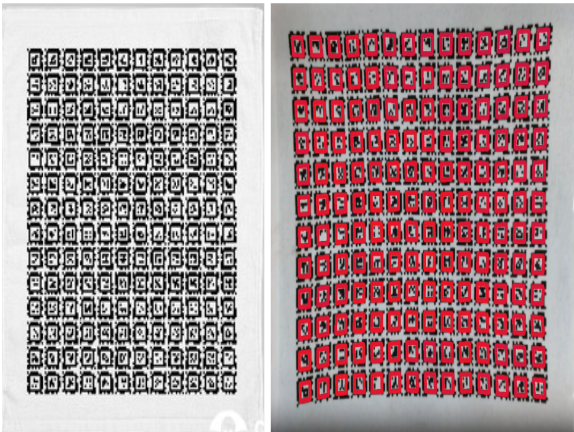
\includegraphics[width=\linewidth]{CLOTH REPORT PICS/Tags.png} % Adjust the image path and extension
\caption{Left- A grid of 168 AprilTags affixed to a cloth for accurate 3D position measurement. Right - The same cloth with detected AprilTags annotated in red by the camera measurement system.}
\label{fig:tags}
\end{figure}

\subsection{Node Count vs. Computational Efficiency}
The number of nodes in the cloth simulation directly affects both the accuracy of the physical model and the computational resources required. Higher node counts improve simulation fidelity by capturing finer details of cloth behavior, but they also increase the computational burden, potentially compromising real-time performance. For our application, maintaining an update rate of approximately 30 frames per second (fps) is deemed sufficient for effective real-time state estimation.

\subsection{CPU vs. GPU Performance Evaluation}
We benchmarked the simulator on both CPU and GPU hardware to determine the optimal compute platform. GPU acceleration is generally beneficial for large-scale problems due to parallelism, while CPUs may outperform for lower node counts. Tests were conducted using an Intel i9-12900 CPU and an Nvidia RTX 4090 GPU. We compared simulation throughput, memory load, and execution time per frame across varying mesh resolutions to guide platform selection for deployment.

\subsection{Experimental Setup}
Our testbed, shown in Fig.~\ref{fig:setup}, consists of a rigid aluminum T-slot frame for consistent cloth drop experiments. The cloth is mounted at four corners, with two adjacent corners released simultaneously to induce a free-fall motion. A total of 238 nodes are simulated, including extra boundary nodes for better edge resolution. GoPro cameras record the cloth's motion, while additional AprilTags on the frame provide static reference points for pose calibration.

\begin{figure}[H]
\centering
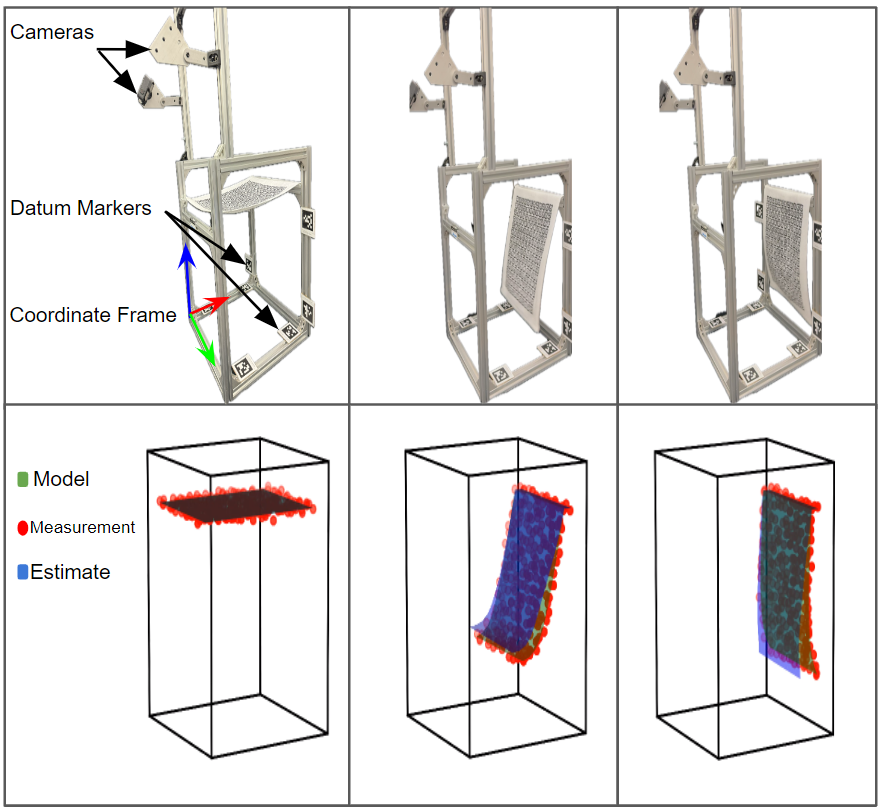
\includegraphics[width=\linewidth]{CLOTH REPORT PICS/Setup.png}
\caption{Experimental setup for dynamic cloth manipulation. Top: The frame with mounted cloth and release mechanism. Bottom: Visualization of the cloth simulation (green), measurement data (red), and EKF estimate (blue).}
\label{fig:setup}
\end{figure}

\subsection{Validation}
We first validate our approach in a simulation-to-simulation (sim2sim) setting. A secondary noisy IPC simulation mimics real-world sensor artifacts, creating a pseudo-real environment to stress test the EKF.

As seen in Fig.~\ref{fig:setup}, we compare the ground truth (green), raw observations (red), and EKF estimates (blue). Evaluation includes covariance matrix convergence and containment of the innovation vector within $3\sigma$ bounds, indicating filter reliability under uncertainty.

%%%%%%%%%%%%%%%%%%%%%%%%%%%%%%%%%%%%%%%%%%%%%%%%%%%%%%%%%%%%%%%%%%%%%%%%%%%%%%%
\section{Results}
\subsection{CPU vs. GPU Computation}

A key consideration in our implementation is whether to run IPC simulations on a CPU or GPU. While GPUs are generally preferred for their massive parallelism, this advantage is not universal. For simulations involving relatively low node counts, such as those used in real-time cloth tracking, the overhead of GPU parallelization can outweigh its benefits. In contrast, CPUs—equipped with fewer but high-performance cores—can outperform GPUs when parallel workload distribution is limited.

To evaluate this trade-off, we benchmarked an Intel i9-12900 CPU against an Nvidia RTX 4090 GPU across varying node counts, as summarized in Table~\ref{tab:ipc_performance_comparison}. With a target of 30fps for realtime applications, we see a node count of 100—near our target performance. In this instance, CPU achieves higher frame rates than the GPU, indicating more effective utilization of available compute resources at this scale.

These findings highlight an important insight: although GPUs dominate high-throughput workloads, our cloth simulation demands—requiring both moderate resolution and real-time speed—are better met by the CPU. For our experiments with 238 nodes, the CPU implementation offers a favorable balance between speed and computational efficiency, making it the preferred platform for our application.

\begin{table}
\centering
\begin{tabular}{|c|c|c|}
\hline
\textbf{\#verts} & \textbf{CPU fps (Intel i9 12900)} & \textbf{GPU fps (RTX 4090)} \\ \hline
9       & 289   & 120 \\ \hline
100     & 69.6  & 40  \\ \hline
1024    & 5.217 & 7.5 \\ \hline
4225    & 0.878 & 3.8 \\ \hline
200000  & NA     & 1.8 \\ \hline
\end{tabular}
\caption{Performance comparison between CPU (Intel i9 12900) and GPU (RTX 4090) for IPC simulations, showcasing the relative efficiency at various node counts.}
\label{tab:ipc_performance_comparison}
\end{table}

\subsection{Sim2Sim Study}

We evaluated our Extended Kalman Filter (EKF) implementation using a simulation-to-simulation (sim2sim) study focused on a cloth drop test under gravity. This analysis addresses key challenges related to state observability and covariance divergence when transitioning from simulated to real-world conditions. Three measurement scenarios were tested:

\begin{itemize}
    \item \textbf{Full State Measurement:} Position and velocity of all nodes are available.
    \item \textbf{Partial State Measurement:} Only position data for all nodes is used.
    \item \textbf{Restricted State Measurement:} Position data is limited to nodes corresponding to observable tags.
\end{itemize}

\begin{figure}[ht]
    \centering
    \begin{subfigure}[b]{0.32\linewidth}
        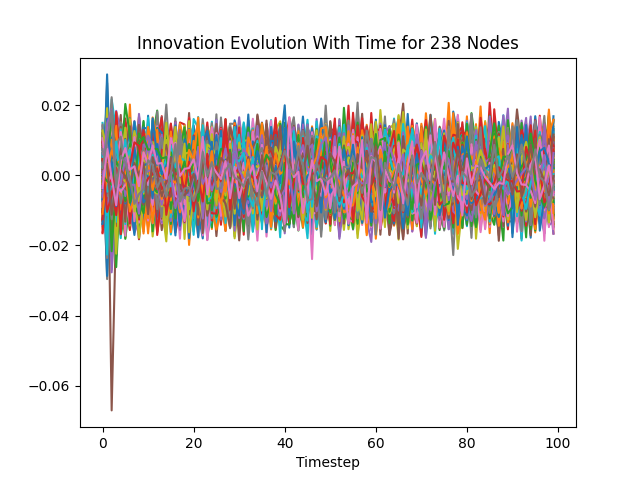
\includegraphics[width=\linewidth]{CLOTH REPORT PICS/innovation 238.jpg}
        \caption{238 nodes, full-state,}
        \label{fig:innovation-238-full}
    \end{subfigure}
    \hfill % optional: add horizontal space between figures
    \begin{subfigure}[b]{0.32\linewidth}
        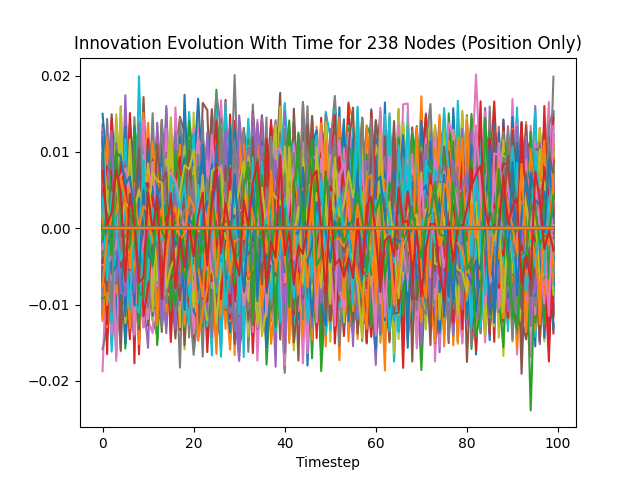
\includegraphics[width=\linewidth]{CLOTH REPORT PICS/innovation 238p.jpg}
        \caption{238 nodes, position only}
        \label{fig:innovation-238-pos}
    \end{subfigure}
    \hfill % optional: add horizontal space between figures
    \begin{subfigure}[b]{0.32\linewidth}
        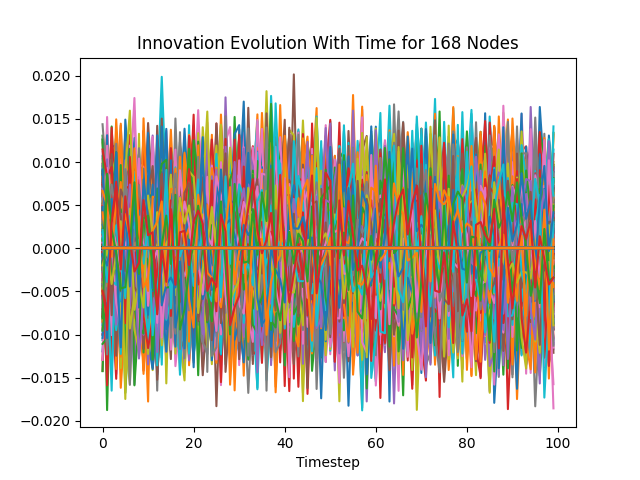
\includegraphics[width=\linewidth]{CLOTH REPORT PICS/innovation 168.jpg}
        \caption{168 nodes, position only}
        \label{fig:innovation-168}
    \end{subfigure}
    \caption{Innovation evolution for position and velocity states of cloth nodes over time, illustrating the variance in measurement updates relative to the predicted state estimates across different configurations.}
    \label{fig:innovations}
\end{figure}

As shown in the innovation plots in Fig.~\ref{fig:innovations}, the EKF demonstrates stable performance across all cases, with innovations remaining bounded and exhibiting low variance over time. This suggests the filter is well-tuned to integrate noisy measurements with the nonlinear cloth dynamics, maintaining consistent estimation accuracy even under reduced observability.

The covariance evolution plots in Fig.~\ref{fig:covariances} further illustrate the EKF’s behavior over time. Initially, the filter exhibits high covariance values, reflecting significant uncertainty in the state estimate. As the EKF incorporates more measurements, these values decrease and stabilize, indicating growing confidence in the state estimation. This trend demonstrates the filter’s capacity to reduce uncertainty and converge toward a consistent estimate as it accumulates information about the system’s dynamics.

A comparison between systems with different node counts (168 vs. 238) highlights the influence of state dimensionality on estimation performance. The 238-node system exhibits slightly decreased noise in the innovation plots, likely due to the added measurements and whole state space being estimated.

As shown in Fig.~\ref{fig:covariance}, the innovation vectors across all scenarios remain within the expected 3-sigma bounds of the position covariance. This consistency underscores the robustness of our EKF, which maintains bounded innovations even under varying levels of measurement granularity and system complexity.

\begin{figure}
    \centering
    \begin{subfigure}[b]{0.32\linewidth}
        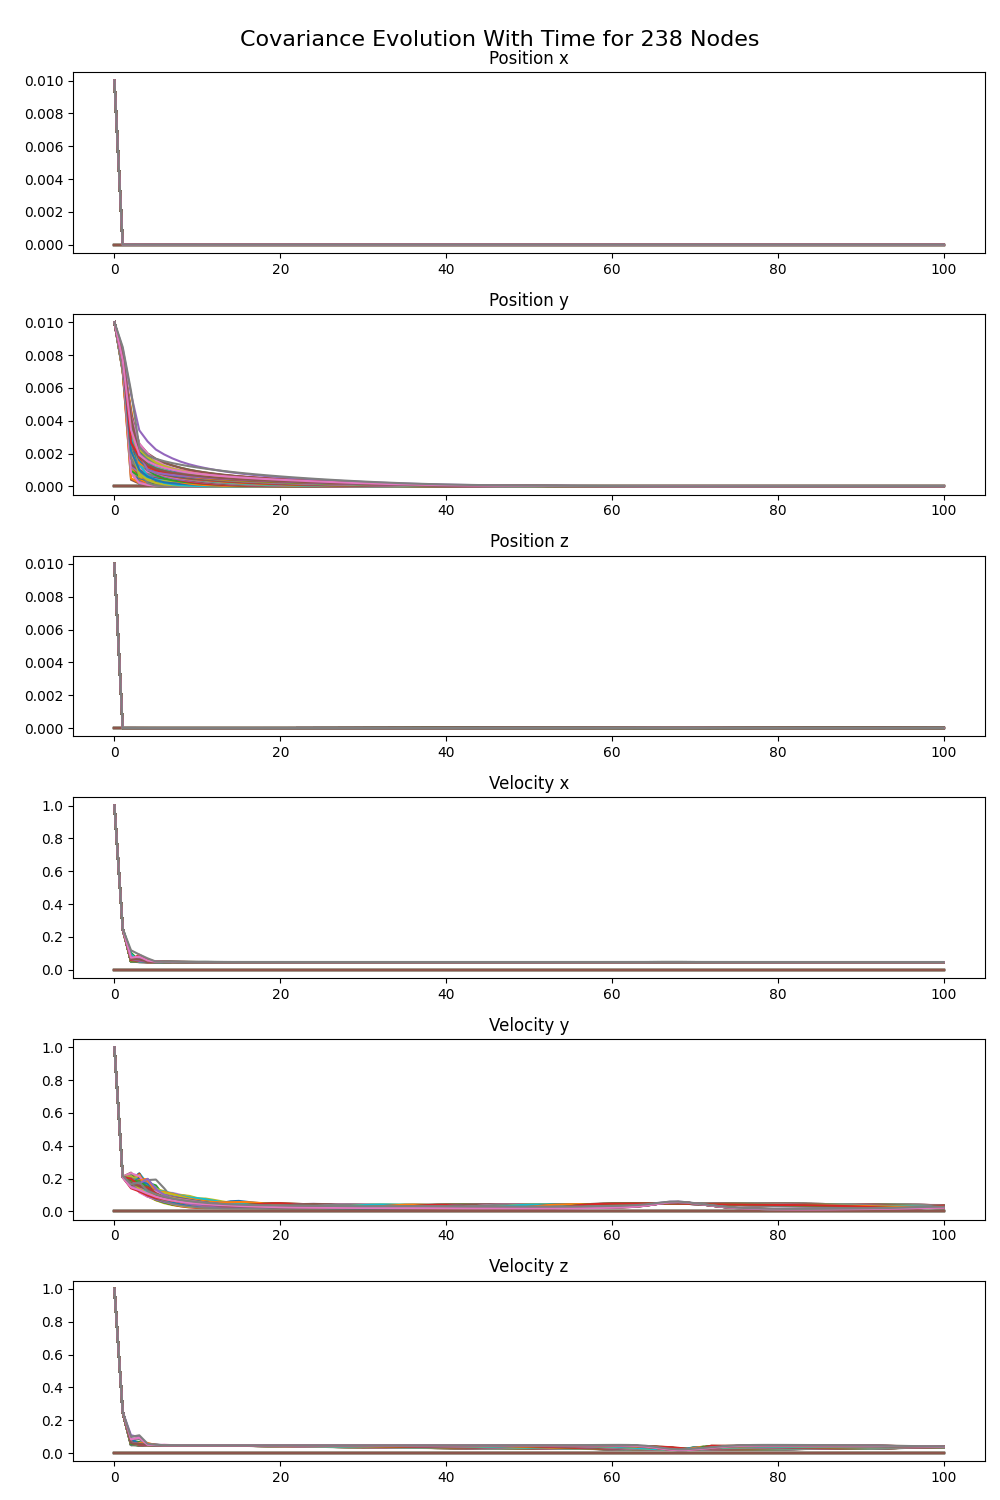
\includegraphics[width=\linewidth]{CLOTH REPORT PICS/covariance 238.jpg}
        \caption{238 nodes, full state}
        \label{fig:covariance-238-full}
    \end{subfigure}
    \hfill % optional: add horizontal space between figures
    \begin{subfigure}[b]{0.32\linewidth}
        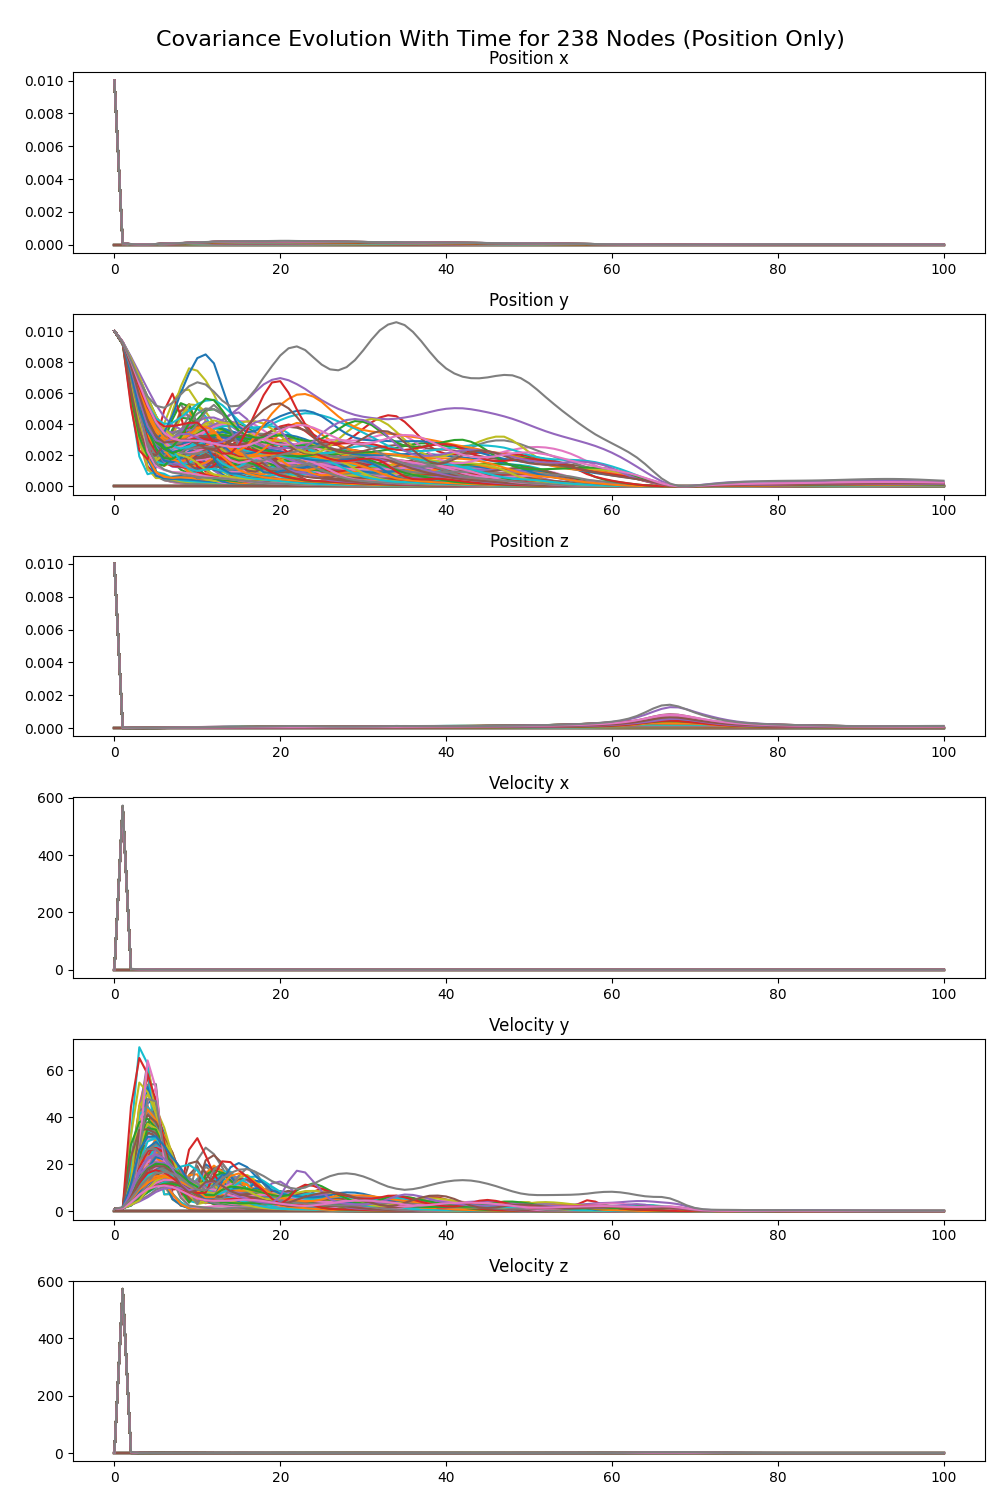
\includegraphics[width=\linewidth]{CLOTH REPORT PICS/covariance 238 p.jpg}
        \caption{238 nodes, position only}
        \label{fig:covariance-238-pos}
    \end{subfigure}
    \hfill % optional: add horizontal space between figures
    \begin{subfigure}[b]{0.32\linewidth}
        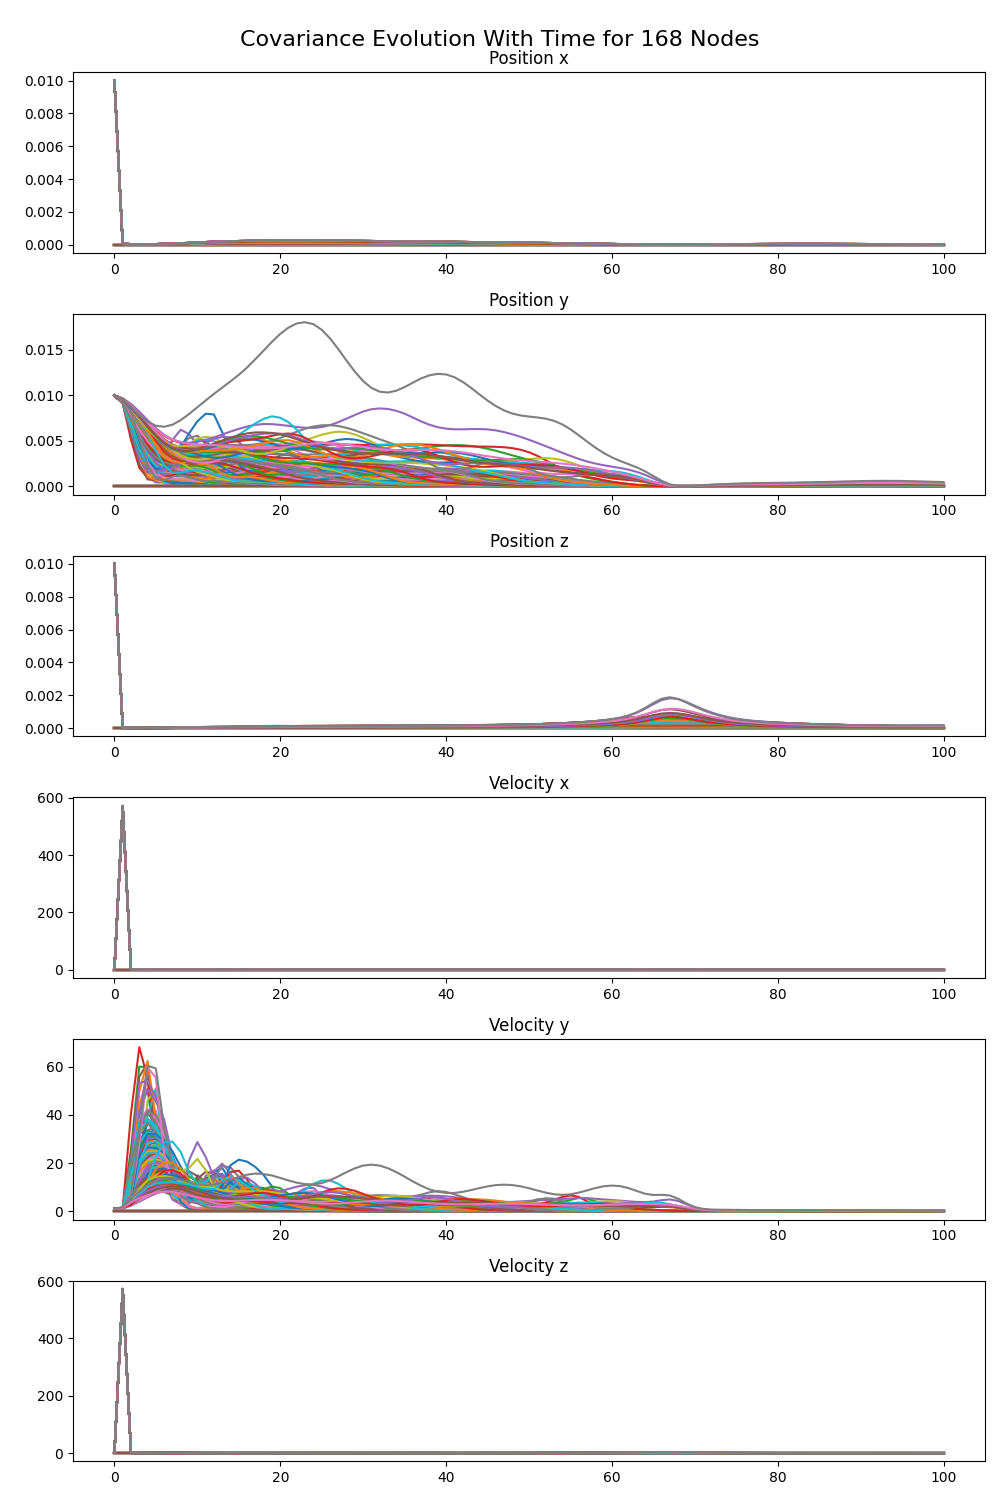
\includegraphics[width=\linewidth]{CLOTH REPORT PICS/covariance 168.jpg}
        \caption{168 nodes, position only}
        \label{fig:covariance-168}
    \end{subfigure}
    \caption{Evolution of covariance values for position and velocity states of cloth nodes in a dynamic manipulation scenario, showcasing the variability in estimation confidence over time for different node configurations and measurement setups.}
    \label{fig:covariances}
\end{figure}

% Inserting a two-column figure
\begin{figure}
\centering
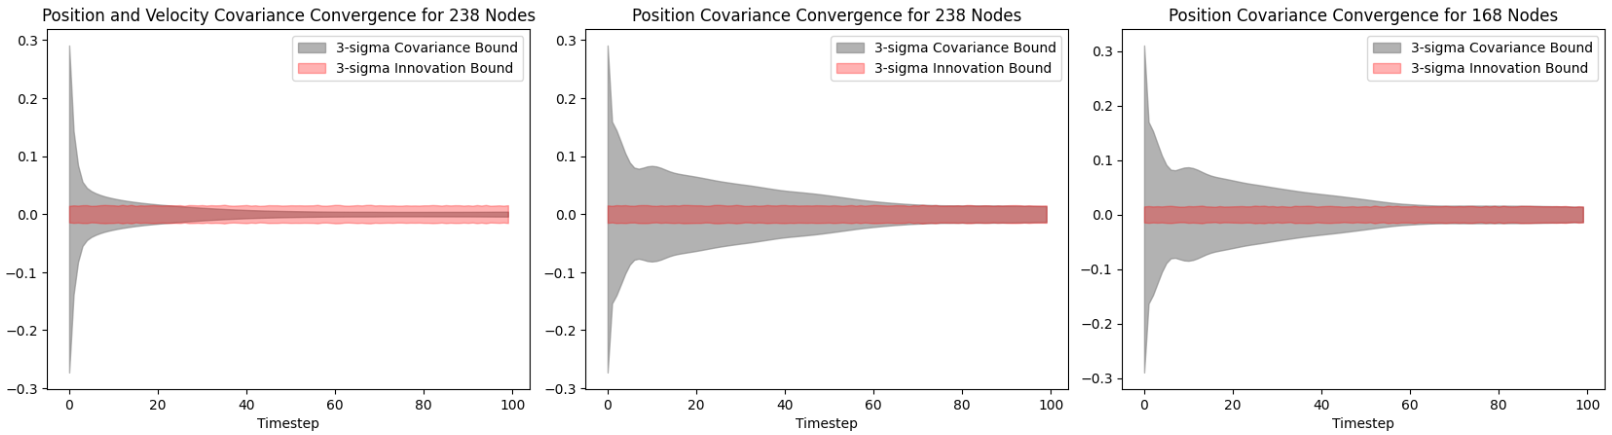
\includegraphics[width=\textwidth]{Covariance Bound.png} % Adjust the image path and extension
\caption{Evaluation of Innovation Vector Boundedness in EKF State Estimation for Cloth Dynamics Across Different Measurement Scenarios. Panel (1) demonstrates the EKF's innovation for all state measurements (positions and velocities) across all nodes, revealing a tightly bounded innovation sequence within the 3-sigma position covariance range. Panel (2) depicts the scenario where only node positions are measured, showing a similarly bounded innovation sequence but with a marginally increased spread. Panel (3) illustrates the filter's performance when limited to the positions of nodes with visible tag information, where the innovation remains bounded yet demonstrates the slowest convergence rate among the three cases.}
\label{fig:covariance}
\end{figure}

Interestingly, the convergence rate of the innovation vector was found to depend on the number of measured state variables. As the quantity of measurement data decreased, convergence slowed. In particular, when only the positions of tagged nodes were observed, the innovation took approximately 50 time steps to stabilize—indicating a clear relationship between measurement density and the speed of state estimation convergence.

These results affirm the EKF's ability to operate reliably within bounded uncertainty, even under limited observability as would be expected in real-world scenarios. While reduced measurements lead to slower convergence, the filter still maintains stability, highlighting the trade-off between measurement richness and estimation responsiveness.

\subsection{Real Cloth Experiment}
To evaluate the performance of our Extended Kalman Filter (EKF) on real-world data, we conducted a drop test using a cloth sample instrumented with AprilTags and tracked using two synchronized GoPro cameras. The EKF was initialized using a physics-based model derived from the IPC simulator, and state estimates were updated using only the observed tag positions corresponding to visible nodes on the cloth.

\subsubsection*{Innovation Consistency}

Figure~\ref{fig:real_cloth_innov} presents the innovation statistics over the duration of the drop. The left subplot shows the innovation values for all observable nodes across time. While there is a high degree of initial variability, the innovations stabilize within a small range by approximately 50 time steps, indicating convergence of the EKF state estimate toward the measured data. 

\subsubsection*{Covariance Validation}

The right subplot in Figure~\ref{fig:real_cloth_innov} compares the 3-sigma range of the innovation vector (red) with the predicted 3-sigma covariance bounds (gray). The innovation remains well within the predicted uncertainty envelope throughout the trajectory, providing strong evidence that the EKF is consistent and well-calibrated. This result confirms that the estimated state uncertainty reasonably captures the actual measurement error, a key criterion for validating probabilistic filters in real-world applications.

\subsubsection*{Observability and Convergence Behavior}

Despite being restricted to partial observations (i.e., tagged nodes only), the EKF successfully maintained bounded innovations and converged to a stable state estimate. The initial transient phase, characterized by larger innovation magnitudes, reflects the time required for the filter to accumulate sufficient information for confident estimation. Notably, this behavior mirrors trends observed in the simulation-based tests, reinforcing the robustness of the EKF under limited measurement conditions.

These results confirm the effectiveness of our pipeline for real-time cloth state estimation using partial visual feedback. Future work will aim to extend this framework with learned observation models and additional sensing modalities (e.g., tactile feedback) to further improve robustness in unstructured environments.

\begin{figure}
    \centering
    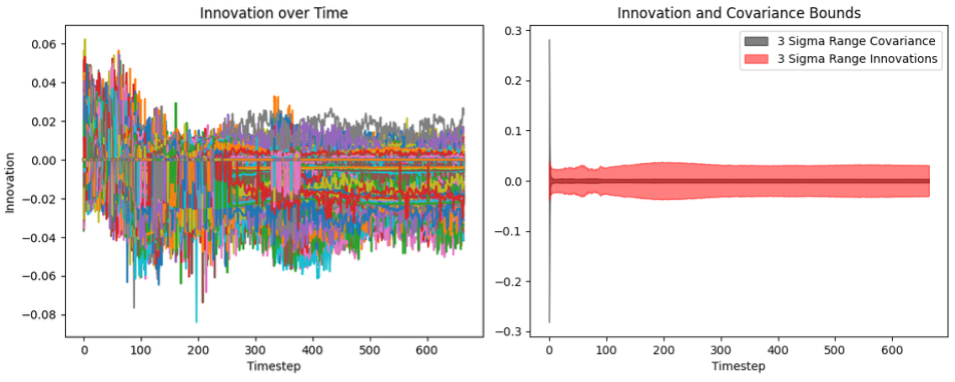
\includegraphics[width=\linewidth]{CLOTH REPORT PICS/real_cloth_data_crop.png}
    \caption{Innovation and covariance analysis for real cloth data during a drop test. \textbf{Left:} Innovation values for all measured nodes over time, showing initial transients followed by convergence to a bounded range. \textbf{Right:} Aggregated 3-sigma innovation bounds (red) compared to the 3-sigma covariance envelope (gray), illustrating that the EKF maintains consistency with the predicted uncertainty bounds across the entire trajectory.}
    \label{fig:real_cloth_innov}
\end{figure}

\section{Future Work}

Building on the successful validation of our EKF framework through both simulation and real-world cloth drop experiments, several promising directions for future research are being pursued.

First, we aim to conduct a systematic observability analysis to quantify how measurement dropout, occlusions, and camera tracking errors affect the filter's performance. Understanding the robustness of the EKF under partial or intermittent observations is critical for deployment in unstructured environments.

Second, we plan to extend our simulation-to-simulation (sim2sim) validation by introducing closed-loop robotic interactions. Unlike passive drop tests, these scenarios will incorporate control inputs from a robotic manipulator, enabling us to assess the filter's responsiveness and accuracy under dynamic, contact-rich conditions.

Third, we will investigate more complex manipulation tasks that involve realistic challenges such as self-occlusion, multi-layer folding, and topological changes in the cloth structure. These tasks will better reflect the demands of real-world applications, such as autonomous laundry folding, bed-making, or dressing assistance.

Ultimately, our long-term objective is to integrate this state estimation framework into a real-time robotic manipulation pipeline. This will require developing robust, latency-tolerant algorithms that can handle noisy sensor data and dynamic interaction forces while maintaining stable cloth tracking. Such capabilities have the potential to transform how robots interact with deformable objects, with applications in domestic robotics, assistive care, textile manufacturing, and beyond.

\section{Conclusion}

This work advances the field of dynamic cloth manipulation by presenting a robust state estimation framework that combines high-fidelity simulation with real-time visual sensing. Leveraging the Codimensional Incremental Potential Contact (CIPC) model, we simulate cloth dynamics with high physical accuracy, enabling realistic modeling of contact-rich scenarios. Visual observations from a dense array of AprilTags are fused with the simulation model using an Extended Kalman Filter (EKF), producing reliable and bounded state estimates.

A study on node count and computational efficiency guided the selection of mesh resolution to balance accuracy and real-time performance. Our custom-built test rig facilitated repeatable cloth drop experiments, enabling controlled validation of the EKF against physical data. Results from both simulation and real-world tests demonstrate the filter’s ability to maintain bounded innovations and converge despite partial observability, validating its robustness and consistency.

Together, these contributions establish a foundation for integrating state estimation into closed-loop robotic manipulation of deformable objects. This framework offers a promising path toward real-time, sensor-informed cloth manipulation in practical applications such as laundry handling, bed-making, and assistive garment dressing.





% %%%%%%%%%%%%%%%%%%%%%%%%%%%%%%%%%%%%%%%%%%%%%%%%%%%%%%%%%%%%%%%%%%%%%%
% \section*{Acknowledgment} %% ASME requests this exact spelling, singular.

% Acknowledge individuals, institutions, or companies that supported the authors in preparing the work. Those mentioned might have provided technical support, insightful comments or conversations, materials used in the work, or access to facilities.






% %%%%%%%%%%%%%  BIBLIOGRAPHY  %%%%%%%%%%%%%%%%%%%%%%%%%%%%%%%%%%%%%%%%%

% \nocite{*} %% <=== delete this line - unless you wish to typeset the entire contents of your .bib file.

% \bibliographystyle{asmejour}   %% .bst file that follows ASME journal format. Do not change.

% \bibliography{asmejour-sample} %% <=== change this to name of your bib file

% %%%%%%%%%%%%%%%%%%%%%%%%%%%%%%%%%%%%%%%%%%%%%%%%%%%%%%%%%%%%%%%%%%%%%%

% %% To omit final list of figures and tables, use the class option [nolists]

% \end{document}
 